%
% LaTeX template at the Institute for Optical Systems (IOS)
%
% Author: Nico Brügel  (nico.bruegel@htwg-konstanz.de)
% Adjusted by Lorenz Bung  (lorenz.bung@htwg-konstanz.de)
% Date: 01.07.2020
%

% Include header
% !TEX root = ../thesis.tex
\documentclass[11pt,a4paper,oneside]{report}		                     

% Mathe
\usepackage{marvosym}		% Package für Euro&Co.
\usepackage{amsfonts}		% Package für Mengensymbole (IN, IR, ...)
\usepackage{amsmath}		% Package für restlichen Mathekram
\usepackage{amssymb}        % math. Symbole und Umgebungen
\usepackage{mathtools}
\usepackage{unicode-math}   % Erlaubt die Mathe Schrift zu setzen

% Use german umlaute
%\usepackage{ngerman}
\usepackage[ngerman]{babel}
%\usepackage[T1]{fontenc}
%\usepackage[utf8]{inputenc}
%\usepackage[english]{babel}

% Zitierung und Literaturverzeichnis
\usepackage{cite}
%\usepackage{apacite}		% Zitierstil
%\usepackage{natbib} 		% Erweiterte zitiermöglichkeiten 
\usepackage{babelbib}		% Übersetzung des Literaturverzeichnisses und der Zitate

% Fonts
\usepackage{fontspec}
\setmainfont[Path=fonts/, BoldFont=swis721-Bold.ttf, ItalicFont=swis721-Italic.ttf, BoldItalicFont=swis721-Bold-Italic.ttf]{swis721.ttf}
\setmonofont[Path=fonts/, BoldFont=CourierNew-Bold.ttf, ItalicFont=CourierNew-Italic.ttf, BoldItalicFont=CourierNew-Bold-Italic.ttf]{CourierNew.ttf}
\setmathfont[Path=fonts/]{CambriaMath.ttf}


% formatting
\usepackage{a4}

% PDF als Cover Hintergrund
\usepackage[firstpage=true]{background}
\usepackage{geometry}
\usepackage{tikz}

% Verbesserte Darstellug der Schriftzeichen und Zwischenräumen
%\usepackage{lmodern}				% Benutze skalierbare Schriftfamilie
%\usepackage[activate]{microtype}

% Heading styles
\usepackage[sf,bf,raggedright]{titlesec}
\titlespacing*{\section}
{0pt}{5.5ex plus 1ex minus .2ex}{4.3ex plus .2ex}
\titlespacing*{\subsection}
{0pt}{5.5ex plus 1ex minus .2ex}{4.3ex plus .2ex}
\titleformat{\chapter}[hang]{\Huge\bfseries}{\thechapter}{15pt}{\Huge\bfseries}

% Header and Footer
\usepackage{fancyhdr}

\fancypagestyle{fancybody}{
	\fancyhf{}
	\fancyhead[L]{\nouppercase{\leftmark}}
	\fancyfoot[C]{\thepage}
}

\fancypagestyle{plain}{
	\fancyhf{}
	\fancyfoot[C]{\thepage}
	\renewcommand{\headrulewidth}{0pt}
}

\pagestyle{fancybody}
\renewcommand{\chaptermark}[1]{\markboth{\normalfont\thechapter.\space#1}{}}

% Absatz einrücken unterdrücken
\setlength{\parindent}{0pt}

% Listings
\usepackage{listings}
\lstset{
	backgroundcolor=\color{lighter-gray},
	xleftmargin=\parindent,
	basicstyle=\ttfamily\footnotesize,
	breaklines=true,
	captionpos=b,
	showspaces=false,
	showstringspaces=false,
	frame=shadowbox,
	rulesepcolor=\color{ll-gray},
	rulecolor=\color{l-gray},
	belowskip=11pt,
}

% Depth of chapters and subsections
\setcounter{tocdepth}{3}
\setcounter{secnumdepth}{3}

% Url line break
\def\UrlBreaks{\do\/\do-}
\def\UrlBigBreaks{\do\:\do\/}

% Links
\usepackage[pdfstartview=FitV, 	% start in 'fit size height'-view
colorlinks=true, 	% Links farbig markieren
linkcolor=black, 	% Interne Links schwarz
citecolor=black, 	% Links zur Literatur schwarz
filecolor=black, 	% Links auf lokale Dateien schwarz
urlcolor=black,   	% Externe Links blau
breaklinks=true, 	% Links umbrechen
linktocpage=true 	% Im Inhaltsverzeichnis sind Seitenzahlen UND Text Links
]{hyperref}

%Move to the right.
\setlength{\hoffset}{5pt}
\setlength{\parskip}{\baselineskip}

% Suppress warning of too small headheight
\headheight13.6pt

% Abkuerzungsverzeichnis
\usepackage[nohyperlinks, printonlyused]{acronym}
\usepackage[mode=buildnew]{standalone}

\usepackage[toc, page]{appendix}


%%%%%%%%%%%%
%% HTWG CI Colors
%%%%%%%%%%%%
\definecolor{htwg-white}{cmyk}{0.0,0.0,0.0,0.0}
\definecolor{htwg-black}{cmyk}{0.0,0.0,0.0,1.0}
\definecolor{htwg-black-90}{cmyk}{0.0,0.0,0.0,0.9}
\definecolor{htwg-black-80}{cmyk}{0.0,0.0,0.0,0.8}
\definecolor{htwg-black-70}{cmyk}{0.0,0.0,0.0,0.7}
\definecolor{htwg-black-60}{cmyk}{0.0,0.0,0.0,0.6}
\definecolor{htwg-black-50}{cmyk}{0.0,0.0,0.0,0.5}
\definecolor{htwg-black-40}{cmyk}{0.0,0.0,0.0,0.4}
\definecolor{htwg-black-30}{cmyk}{0.0,0.0,0.0,0.3}
\definecolor{htwg-black-20}{cmyk}{0.0,0.0,0.0,0.2}
\definecolor{htwg-black-10}{cmyk}{0.0,0.0,0.0,0.1}
\definecolor{htwg-soft-blue}{cmyk}{0.1,0.0,0.0,0.1}
\definecolor{htwg-dark-blue}{rgb}{0.165, 0.22, 0.29}
\definecolor{htwg-teal}{cmyk}{1.0,0.0,0.5,0.0}


% Set variables used in cover, title, abstract and affidavit.
\newcommand{\ausgabedatum}{01.05.2020}
\newcommand{\abgabedatum}{31.07.2020}
\newcommand{\autor}{Lorenz Bung}
\newcommand{\matrikelnummer}{295261}
\newcommand{\autorStrasse}{Banater Str. 9}
\newcommand{\autorPLZ}{78467}
\newcommand{\autorOrt}{Konstanz}
\newcommand{\autorEmail}{lorenz.bung@htwg-kostanz.de}
\newcommand{\autorGeburtsort}{Konstanz}
\newcommand{\autorGeburtsdatum}{26.06.1997}
\newcommand{\prueferA}{Prof. Dr. Georg Umlauf}
\newcommand{\prueferB}{Simon Schmei{\ss}er, M. Sc.}
\newcommand{\firma}{Isys Vision GmbH}
\newcommand{\studiengang}{Angewandte Informatik}


\newcommand{\thema}{Rekonstruktion von Meshes für industrielles Bin-Picking und Depalettieren}

\newcommand{\schlagworte}{Meshrekonstruktion, Robotik, Geometrisches Modellieren, ROS, PCL, Punktwolke}

\begin{document}

% Include title pages
% !TEX root = ../thesis.tex
\begin{titlepage}

\vspace*{-2.5cm}

\begin{figure}[h]
\hspace*{-2cm}

\includegraphics[height=2cm]{title/HTWG-Logo_en_300dpi.png}
\hspace*{4cm}
\includegraphics[height=2cm,]{title/IOS_Logo2016_lettering_en.png}


\end{figure}

\vspace{2cm}

\begin{center}
	 \LARGE{
		\textbf{\thema} \\[5cm]
	}
	\Large{
		\textbf{\autor}} \\[5.5cm]
	\large{
		\textbf{Konstanz, \abgabedatum} \\[2.3cm]
	}
	
	\Huge{
		\textbf{{\sf BACHELORARBEIT}}
	}
\end{center}

\end{titlepage}

% !TEX root = ../thesis.tex
\thispagestyle{empty}
{
\setlength{\parskip}{1cm}
        \begin{center}
        \textbf{\Huge BACHELORARBEIT}\\[15ex]

        \textbf{zur Erlangung des akademischen Grades}

        \textbf{\Large Bachelor of Science (B. Sc.)}

        \textbf{an der}

        \textsf{\huge Hochschule Konstanz}\\
        {\small Technik, Wirtschaft und Gestaltung}

        \textsf{\Large Fakultät Informatik} \\
        Studiengang \studiengang\\[15ex]
        
        \begin{tabular}{p{3cm} p{7cm}}
        Thema: & \thema\\[1cm]
        Kandidat: & \autor \\
        	                  & \autorStrasse \\
                          & \autorPLZ\ \autorOrt \\[1cm]
        1. Prüfer: & \prueferA \\
        2. Prüfer: & \prueferB \\[1cm]
        Ausgabedatum: & \ausgabedatum \\
        Abgabedatum: & \abgabedatum \\
        \end{tabular}
        \end{center}
}

\newpage


% Set page numbering to roman
\pagenumbering{Roman}

% Include abstract and affidavit
% !TEX root = ../thesis.tex
\thispagestyle{plain}
\chapter*{Ehrenwörtliche Erklärung}
\label{ch:affidavit}

Hiermit erkläre ich,
\textit{\autor, geboren am \autorGeburtsdatum\ in \autorGeburtsort}, dass ich\\

\begin{tabular}{lp{12cm}}
(1) & meine Bachelorarbeit mit dem Titel \\[1em]
& \textbf{\thema} \\[1em]
& bei \firma\ unter Anleitung von \prueferA\ und \prueferB\ selbständig und ohne fremde Hilfe angefertigt und keine anderen als die angeführten Hilfen benutzt habe;\\[1em]
(2) & die Übernahme wörtlicher Zitate, von Tabellen, Zeichnungen, Bildern und
Programmen aus der Literatur oder anderen Quellen (Internet) sowie die Verwendung
der Gedanken anderer Autoren an den entsprechenden Stellen innerhalb der Arbeit
gekennzeichnet habe;\\[1em]
(3) & dass die eingereichten Abgabe-Exemplare in Papierform und im PDF-Format vollständig übereinstimmen.
\end{tabular}

\vspace*{1cm}

\noindent
Ich bin mir bewusst, dass eine falsche Erklärung rechtliche Folgen haben wird.\\

\vspace*{1cm}

\noindent
Konstanz, \abgabedatum \hfill \begin{tabular}{c} \\ \\ \rule{5cm}{1pt} \\ (Unterschrift)\end{tabular}

\newpage

% !TEX root = ../thesis.tex
\thispagestyle{plain}
\chapter*{Abstract}
\label{ch:abstract}


\begin{center}
	\begin{tabular}{p{3.2cm}p{9.6cm}}
		Thema: & \thema \\[1ex]
		% & \\
		Bachelorkandidat: & \autor \\[1ex]
		% & \\
		Betreuer: & \prueferA \\%[.5ex]
		 & Institut für Optische Systeme\\[1ex]
		 & \prueferB \\%[.5ex]
		 & \firma \\[1ex]
		% & \\
		Abgabedatum: & \abgabedatum \\[1ex]
		% & \\
		Schlagworte: & \schlagworte \\
		% & \\
	\end{tabular}
\end{center}


Describe the objective and results of this thesis in a few words.
Typically one page.

In dieser Arbeit werden verschiedene Ansätze zur Rekonstruktion von Meshes aus 3D-Punktwolken analysiert, miteinander verglichen und bewertet.
Die erste Methode ist YAK, eine Variante von Kinect Fusion, bei der ein Truncated Signed Distance Field zum Einsatz kommt.
Der zweite Ansatz ist, ein einzelnes Teil mithilfe einer beweglichen Kamera am Roboterarm aus mehreren Posen einzuscannen und so ein Gesamtbild zu erhalten.
Im dritten Ansatz wird eine 

\newpage

% !TEX root = ../thesis.tex
\thispagestyle{plain}
\chapter*{Extended Abstract}
\label{ch:extended-abstract}

\begin{refsection}

\begin{center}
	\begin{tabular}{p{3cm}p{10cm}}
		Thema: & \thema \\[1ex]
		Kandidat: & \autor \\[1ex]
		Betreuer: & \prueferA \\
		 & Institut für Optische Systeme\\[1ex]
		 & \prueferB \\
		 & \firma \\[1ex]
		Abgabedatum: & \abgabedatum \\[1ex]
		Schlagworte: & \schlagworte \\[1ex]
	\end{tabular}
\end{center}


\section*{Einleitung}

Robotik spielt im industriellen Bereich eine größer werdende Rolle.
Insbesondere das sogenannte Bin-Picking, also das autonome Greifen unsortierter Teile gewinnt zunehmend an Relevanz.
Zur Erkennung der Objekte werden dabei in vielen Fällen CAD-Modelle benötigt, welche jedoch nicht immer vorliegen.
Die Rekonstruktion aus aufgenommenen 3D-Daten bietet daher eine einfache Möglichkeit, diese zu erhalten.
Es wurden verschiedene Ansätze dafür analysiert, verglichen und bewertet.


\section*{Methodik}

Die Pipeline wurde in großen Teilen auf Basis der Point Cloud Library \cite{rusu2011pcl} implementiert.
Um größtmögliche Flexibilität zu erreichen, wurde das Robot Operating System \cite{quigley2009ros} für die Interaktion mit dem Programm eingesetzt.
Zur Aufnahme der 3D-Punktwolken wurden Kameras von Ensenso \cite{ensensoWebsite} verwendet.

Die Segmentierung der Punktwolke wurde sowohl im 3D durch Euclidean Cluster Extraction und Region Growing getestet, als auch im zweidimensionalen Grauwertbild mithilfe des Watershed-Algorithmus.

Um Punktwolken aneinander auszurichten, wurde zunächst eine globale Registrierung durch 4-Point Congruent Sets \cite{aiger2008fpcs} durchgeführt.
Diese wurde anschließend mit Iterative Closest Point \cite{besl1992method} lokal optimiert.

Zur Triangulierung wurde der Poisson-Algorithmus \cite{kazhdan2006poisson} verwendet. Anschließend wurden alle Faces aus dem Mesh entfernt, welche eine gewählte Distanz von der Punktwolke überschritten.


\section*{Ergebnisse}

Zur Evaluation wurde die Cloud-Mesh-Distanz zwischen den Vertices des generierten Meshs und den Faces des Referenzobjekts bestimmt.
Außerdem wurde die inverse Cloud-Mesh-Distanz errechnet, um die Vollständigkeit zu überprüfen.

\begin{figure}[H]
    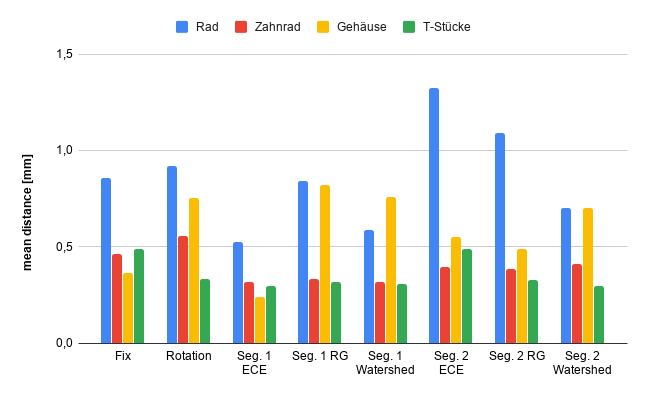
\includegraphics[width=0.49\textwidth]{images/segmentation/meanDistance1.png}
    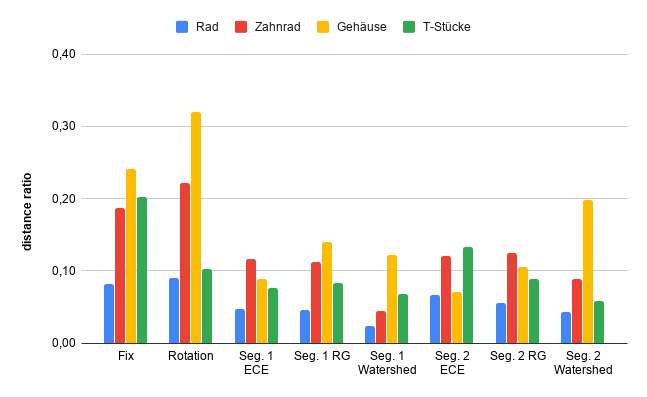
\includegraphics[width=0.49\textwidth]{images/segmentation/ratio.png}
    \caption{Cloud-Mesh-Distanz und Distanzverhältnis verschiedener Testobjekte}
    \label{fig:ex-abstract-distances}
\end{figure}

Es hat sich gezeigt, dass eine Rekonstruktion aus mehreren Aufnahmen eines einzelnen Objekts aus verschiedenen Perspektiven die höchste Qualität erreicht.
In \autoref{fig:ex-abstract-distances} sind die Cloud-Mesh-Distanz von Rekonstruktion zu Referenzobjekt sowie das Distanzverhältnis zu sehen.

Weiterhin ist aufgefallen, dass eine gute Rekonstruktion nur bei korrekter Segmentierung möglich ist.
Bei Untersegmentierung der Punktwolke müssen viele Cluster verworfen werden, während eine korrekte Registrierung bei einer Übersegmentierung oft nicht möglich ist.
Die Wahl der besten Segmentierungsmethode ist abhängig von der Objektform und -größe.

%TODO

\printbibliography[heading=subbibliography]

\end{refsection}
\newpage

%% !TEX root = ../thesis.tex
\thispagestyle{plain}
\chapter*{Danksagung}
\label{ch:danksagung}

Ich möchte mich herzlich bei Simon Schmeißer von der Firma Isys Vision GmbH für die Betreuung bedanken - ohne ihn wäre diese Bachelorarbeit nicht möglich gewesen.

Auch allen weiteren Mitarbeitern von Isys Vision möchte ich für das Ermöglichen der Arbeit sowie das freundliche Arbeitsumfeld danken.

Weiterhin gilt mein Dank den Mitgliedern des Instituts für Optische Systeme, da sie mich bei meiner Tätigkeit am Institut maßgeblich auf diese Arbeit vorbereitet haben.

\setlength{\parskip}{0pt plus1pt}	% Keine Zeilenumbrüche in der Gliederung
% Include table of contents
\tableofcontents
\newpage
\setlength{\parskip}{\baselineskip}	% Zeilenumbrüche wieder aktivieren

\renewcommand{\headheight}{14pt}

% !TEX root = ../thesis.tex
\thispagestyle{plain}
\chapter*{Abkürzungsverzeichnis}
\label{ch:acronyms}

\begin{acronym}[KinFu]
	\acro{PCL}{Point Cloud Library}
	\acro{ROS}{Robot Operating System}
	\acro{KinFu}{Kinect Fusion}
	\acro{YAK}{Yet Another Kinect Fusion}
	\acro{ICP}{Iterative Closest Point}
	\acro{4PCS}{Four-Points Congruent Sets}
	\acro{TSDF}{Truncated Signed Distance Field}
	\acro{OpenGR}{Open Global Registration}
	\acro{VVM}{Vertex-Vertex-Mesh}
	\acro{LUT}{Lookup Table}
	\acro{CUDA}{Compute Unified Device Architecture}
	\acro{ECE}{Euclidean Cluster Extracion}
	\acro{RoI}{Region of Interest}
	\acro{MSE}{Mean Squared Error}
	\acro{KNN}{K Nearest Neighbors}
\end{acronym}

\newpage

% Aktuelle Seitenzahl in einem Zähler speichern
% -> römische Seitennummerierung soll durchgängig
% sein und wird nachher wieder aufgegriffen werden.
% --------------------------------------------------------
\newcounter{anhang}
\setcounter{anhang}{\value{page}}

% Set page numbering to arabic
\pagenumbering{arabic}

% Include the chapters
% ---------------------------------------------------------------------------
% !TEX root = ../thesis.tex

\chapter{Einleitung}
\label{ch:einleitung}


\section{Motivation}
\label{sec:motivation}

Robotik im industriellen Kontext spielt in den letzten Jahren eine immer größer werdende Rolle für die Wirtschaft.
Insbesondere das autonome Greifen von unsortierten Teilen (sogenanntes Bin-Picking) durch einen Roboter kann viele Prozesse beschleunigen und somit wertvolle Zeit und Ressourcen sparen.

Zum Greifen der Objekte müssen jeweils Position und Orientierung bekannt sein.
Für die dabei durchgeführte Erkennung sind in vielen Fällen CAD-Modelle der Objekte erforderlich, beispielsweise für den ``surface based matching''-Algorithmus \cite{drost2014recognition}.
Dies stellt häufig ein Problem dar, da diese aus verschiedenen Gründen nicht vorhanden sein können.
Etwa können für Objekte im aktuellen Fertigungszustand keine Modelle existieren.
Ein weiterer Grund für fehlende CAD-Daten ist, dass diese aus organisatorischen Gründen schwer zu bekommen sind, beispielsweise wenn nur eine Weiterverarbeitung eines zugelieferten Bauteils stattfindet.

Neben fehlenden sind auch häufig falsche Modelle ein Problem.
So kann es vorkommen, dass das tatsächlich vorhandene Produkt fertigungsbedingte Abweichungen von den existierenden Daten aufweist und Teile daher nicht korrekt erkannt werden können.

Bei Bin-Picking-Anwendungen sind in vielen Fällen 3D-Kameras am Roboter verbaut.
Um schnell eine korrekte Darstellung der Objekte zu erhalten ist es eine Möglichkeit, die aufgenommenen 3D-Daten zur Generierung eines CAD-Modells zu verwenden.
Insbesondere bei wechselnden Produktkonfigurationen vereinfacht dies den Anwendungsprozess enorm.



\section{Zielsetzung}
\label{sec:zielsetzung}

In vielen Fällen liefern 3D-Kameras Daten in Form einer Punktwolke, eine Darstellung, auf die in \ref{subsec:punktwolken} genauer eingegangen wird.
Zur Rekonstruktion eines CAD-Modells aus einer solchen Punktwolke gibt es drei verschiedene Ansätze:

\begin{enumerate}
\item Eine am Roboterarm befestigte Kamera nimmt das Objekt aus verschiedenen Winkeln auf.
Die Kameraposition ist durch die Pose des Roboters gegeben.
\item Eine fest montierte, unbewegliche Kamera nimmt mehrere Aufnahmen eines Objekts auf, das zwischen den Aufnahmen bewegt wird.
Da die Position des Teils unbekannt ist, muss diese geschätzt werden.
\item Durch eine unbewegliche Kamera wird eine einzelne Aufnahme einer Kiste mit Objekten derselben Art aufgenommen.
Die unterschiedliche Orientierung der Objekte innerhalb der Kiste führt zu Daten aus mehreren Perspektiven.
\end{enumerate}

Ziel der Arbeit ist es, geeignete Lösungen für die verschiedenen Ansätze zu entwickeln sowie die unterschiedlichen Rekonstruktionsmöglichkeiten zu implementieren.

Weiterhin sollen die Ergebnisse untereinander und mit bereits bestehenden Algorithmen verglichen werden.
Dieser Vergleich soll sowohl bezüglich der wichtigsten Eigenschaft der Qualität, als auch auf Basis untergeordneter Faktoren wie Geschwindigkeit der Algorithmen und Nutzungskomfort der Ansätze stattfinden.



\section{Anwendungsbereich}
\label{sec:anwendungsbereich}

Entwurf, Implementierung und Evaluation der Ergebnisse finden mithilfe des proprietären Softwarepakets Mikado \cite{mikadoWebsite} statt, einem Projekt von isys vision GmbH \cite{isysWebsite}.
Zur Erfassung der Bilddaten kommen 3D-Kameras von Ensenso \cite{ensensoWebsite} zum Einsatz.

% !TEX root = ../thesis.tex

\chapter{Grundlagen}
\label{ch:grundlagen}

Zum Verständnis des Themas der Arbeit ist die Erklärung einiger Grundlagen notwendig.
In \ref{sec:3d-bilder} und \ref{sec:meshrepr} werden zunächst einmal wichtige Grundbegriffe und Datenstrukturen erläutert, die bei der Arbeit mit 3D-Daten auftreten.
Anschließend werden die verwendeten Bibliotheken \ac{PCL} und \ac{ROS} erklärt, welche zur Datenverarbeitung bzw. zur Robotersteuerung verwendet wurden.
%TODO Remove ROS
Außerdem sind selbstverständlich die bereits bestehenden Elemente des Mikado-Projekts relevant, da diese Arbeit fundamental darauf aufbaut.


\section{Aufnahme und Speicherung von 3D-Bildern}
\label{sec:3d-bilder}

%TODO Tiefergehende / fundiertere Informationen zur Aufnahme. Quellen fehlen.
Zur Aufnahme von 3D-Bilddaten gibt es mehrere verschiedene Möglichkeiten.
Ein LIDAR-System sendet beispielsweise mehrere Lichtstrahlen in verschiedene Richtungen, die anschließend Informationen über die Entfernung zu einem Objekt in diesem Punkt liefern.
Eine Stereokamera liefert im Gegensatz dazu zwei Bilder, die anschließend durch spezielle Software zu einem dreidimensionalen Bild zusammengesetzt werden.
Eine weitere Möglichkeit besteht darin, ein bestimmtes Muster auf die Umgebung zu projezieren, dieses dann aus einer anderen Perspektive aufzunehmen und aus der räumlichen Verzerrung des Musters die Tiefe zu errechnen.

Die so gewonnenen Informationen lassen sich durch mehrere verschiedene Datenmodelle repräsentieren.


\subsection{Tiefenbild}
\label{subsec:tiefenbild}

Ein Tiefenbild ist eine einfache Möglichkeit, in einem zweidimensionalen Bild zusätzlich Informationen über die Entfernung der Kamera zu Objekten abzuspeichern.
Diese Technik ist unter Anderem aus der Computergrafik bekannt, wo sie beim Z-Buffering Anwendung findet \cite[S.32]{catmull1974subdivision}.
Dabei werden sowohl das aufgenommene Bild, aber zusätzlich auch ein 2D-Array mit der Tiefeninformation des zugehörigen Pixels gespeichert.
Ein Beispiel für den Zusammenhang zwischen diesen beiden Komponenten ist in \autoref{fig:depth_map} dargestellt.

So kann das originale 2D-Bild um eine dritte Dimension erweitert werden, wodurch sich beispielsweise dreidimensionale Formen modellieren oder rekonstruieren lassen \cite{arsalan2017synthesizing}.
Auch in der 3D-Fotografie finden Tiefenbilder Anwendung \cite{redert2006philips}.

\begin{figure}[ht]
	\centering
	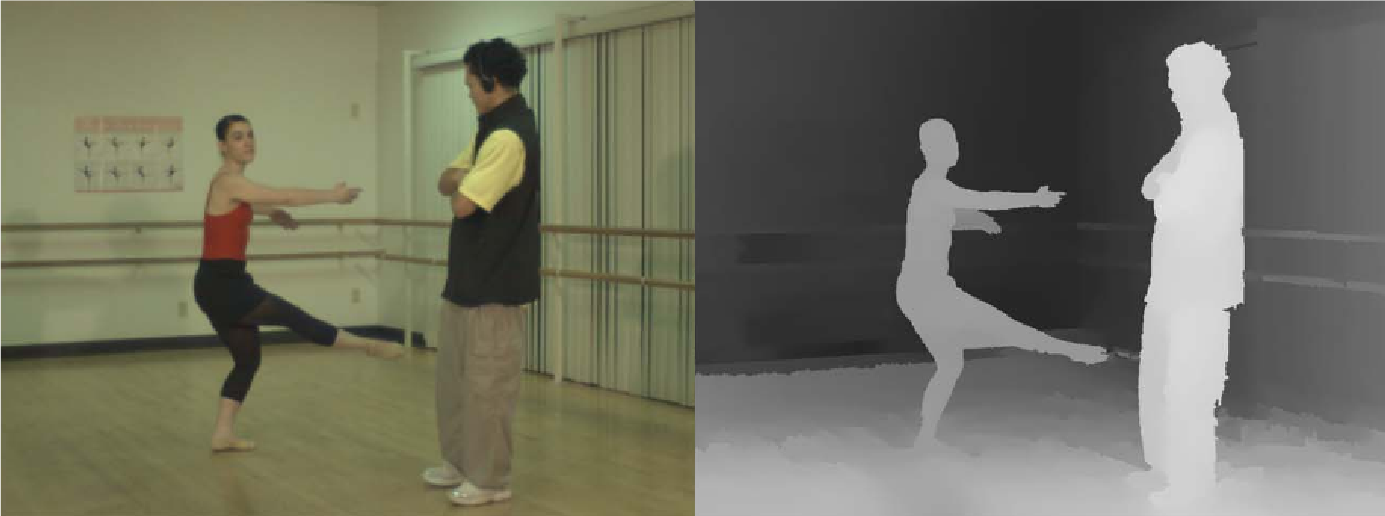
\includegraphics[width=0.66\textwidth]{images/depth_map.png}
	\caption{2D-Farbbild und zugehöriges Tiefenbild. Entnommen aus \cite[S.649]{muller2010depth}}
	\label{fig:depth_map}
\end{figure}

Tiefenbilder haben im Vergleich zu anderen möglichen Datenmodellen den Vorteil, dass 2D-Bilder sehr einfach um zugehörige Tiefeninformationen erweitert werden können.
Jedoch gibt es auch einige Nachteile, die nicht umgangen werden können:

\begin{itemize}
\item Die 3D-Daten sind ausschließlich aus der Kameraperspektive vorhanden.
Um Informationen aus einer anderen Perspektive zu erhalten, muss erst aufwändig umgerechnet werden.
\item Da (in den meisten Fällen) nur ein zweidimensionales Array für die Tiefeninformation angelegt wird, können nur die Entfernungen zu den der Kamera nächsten Objekte gespeichert werden.
Verdeckte, reflektierende oder durchsichtige Oberflächen können nicht gespeichert werden.
\item Das Array ist an die Auflösung der Kamera gebunden.
Insbesondere bei großer Entfernung zu Objekten werden diese aufgrund des Bildwinkels sehr schlecht abgetastet, was später zu Aliasing-Effekten führen kann.
\item Die Bittiefe der Werte im Array kann - je nach gewünschter Auflösung - zu niedrig sein, bzw. muss erhöht werden.
Eine typische Farbtiefe eines Grauwertbilds von 8 Bit repräsentiert beispielsweise nur $2^8 = 256$ Stufen - was schnell zu wenig wird.
Insbesondere bei hoher notwendiger Auflösung im nahen Bereich, aber gleichzeitig vorhandenen weit entfernten Objekten kann dies zum Problem werden.
\end{itemize}


\subsection{Voxel Grid}
\label{subsec:voxel-grid}

Bei einem als Bitmap vorliegendes 2D-Bild werden die Bilddaten diskretisiert in einem zweidimensionalen Array $I$ gespeichert.
Mit einer Bittiefe $b$, einer Bildhöhe $i$ und einer Bildbreite $j$ ergibt sich damit folgende Matrix:

$$I = \begin{pmatrix}
v_{11} & v_{12} & v_{13} & \cdots\\
v_{21} & v_{22} & v_{23} & \cdots\\
v_{31} & v_{32} & v_{33} & \cdots\\
\vdots & \vdots & \vdots & \ddots
\end{pmatrix}, v_{ij} \in [0; 2^b) \wedge b, i, j \in \mathbb{N}^+$$

Dieses Prinzip lässt sich einfach auf den dreidimensionalen Raum erweitern.
Die so erhaltene Datenstruktur nennt sich Voxel Grid.
Als Voxel bezeichnet man somit eine einzelne Datenzelle im 3D-Array, also das dreidimensionale Äquivalent zum Pixel.

Voxel Grids finden in vielen Bereichen Anwendung, zum Beispiel in der Medizin \cite{van2008hippocampus, klein2009elastix, mohanty2012secure, roche1999towards} oder Geographie \cite{chmielewski2017estimating}.
Auch zum Downsampling von Punktwolken werden sie verwendet \cite{pclVoxelGrid}. %TODO Zu Punktwolken / Implementierung...

Gegenüber einem Tiefenbild hat ein Voxel Grid den inhärenten Nachteil, dass Speicherplatz für jeden Voxel benötigt wird.
Dies führt schnell zu großem Speicherbedarf $M$, da dieser kubisch zur Auflösung $r$ steigt: $M = r_x * r_y * r_z * b$ bei Bittiefe $b$.
Da der Speicher bereits bei der Initialisierung reserviert werden muss, ist die Änderung der Auflösung oder der Größe des abgedeckten Raumes unmöglich.
In diesem Fall müssen ein neues Voxel Grid (mit der neuen Auflösung bzw. Größe) angelegt und sämtliche Daten kopiert werden.

Zur Reduzierung des großen Speicherbedarfs werden deswegen häufig Baumstrukturen (sogenannte Octrees) eingesetzt.
Dabei wird der Raum in 8 Voxel geteilt, welche jeweils ein Blatt des Baumes darstellen.
Ist der Voxel gefüllt, wird er wieder entsprechend in 8 Untervoxel geteilt.
Dies wird wiederholt, bis die gewünschte Auflösung erreicht oder eine bestimmte Tiefe im Baum erreicht ist.
Szenen, die große Unterschiede in der Auflösung aufweisen oder viele leere Voxel beinhalten, brauchen so deutlich weniger Speicherplatz.

Ein Vorteil im Vergleich zum Tiefenbild ist jedoch, dass die Abhängigkeit von der Kameraperspektive wegfällt.
Dadurch können hier auch Objekte modelliert werden, die im Tiefenbild durch eine Verdeckung versteckt wären.
Desweiteren ist der Raum einheitlich diskretisiert.
Dies kann je nach Szene und Kameraposition sowohl ein Vor- als auch ein Nachteil sein:
Bei einem Tiefenbild nimmt der Abstand der Messpunkte mit der Tiefe ab.
Ist die Entfernung zwischen Objekt und Kamera gering, werden diese mit einer deutlich besseren Auflösung abgetastet als sehr weit entfernte Objekte.
Im Voxel Grid werden Objekte jedoch überall gleich abgetastet.
Dies führt zu verbesserter Auflösung bei entfernten und zu schlechterer Auflösung bei nahen Objekten.


\subsection{Punktwolken}
\label{subsec:punktwolken}

Ein weiteres häufig verwendetes Datenmodell ist eine Punktwolke.
Als Punktwolke bezeichnet man eine Menge $M \subset \mathbb{R}^3$ von Punkten im (mindestens) dreidimensionalen Raum.
Zusätzlich zur räumlichen Information können auch noch weitere Daten pro Punkt gespeichert sein, wie RGB-Werte, Normalen, Genauigkeit oder Objektklasse (falls schon eine Segmentierung vorgenommen wurde).
Dadurch gilt:
$$M = \begin{pmatrix}
p_x^1 & p_y^1 & p_z^1 & \cdots\\
p_x^2 & p_y^2 & p_z^2 & \cdots\\
p_x^3 & p_y^3 & p_z^3 & \cdots\\
\vdots & \vdots & \vdots & \ddots
\end{pmatrix}$$

\begin{figure}[ht]
	\centering
	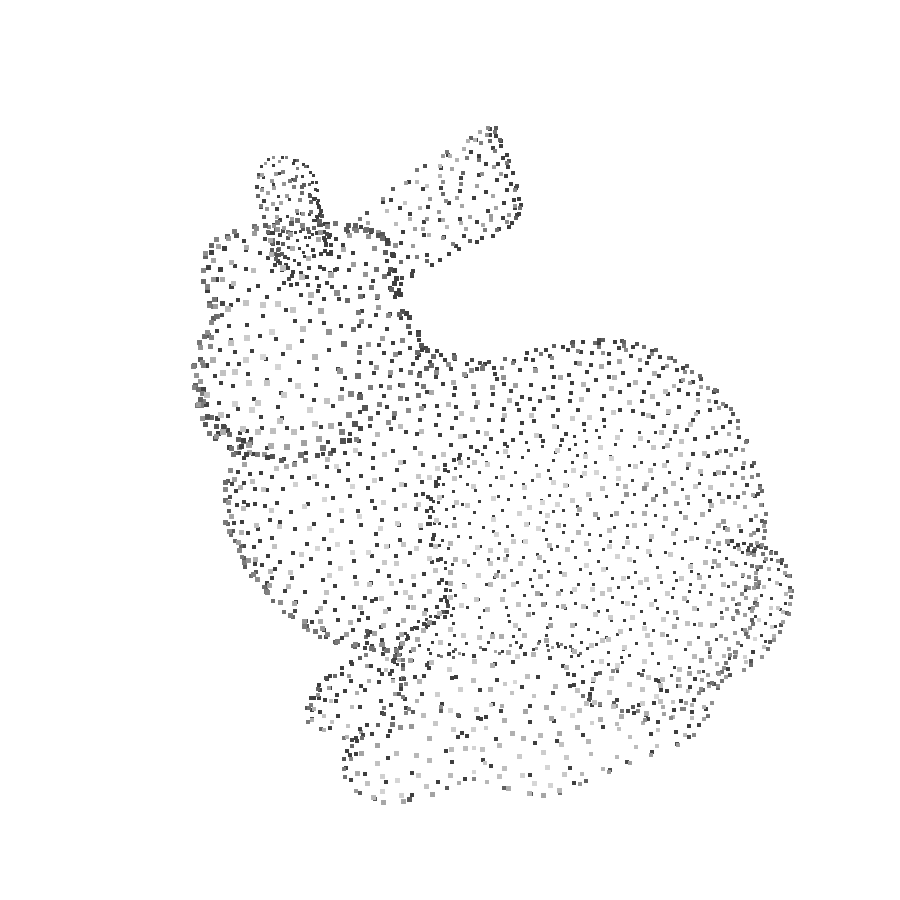
\includegraphics[width=0.66\textwidth, frame]{images/bunny_pcd.png}
	\caption{Punktwolke des Stanford Bunny \cite{stanfordbunny}}
	\label{fig:bunny_pcd}
\end{figure}

Die Nutzung von Punktwolken bringt im Vergleich zu anderen 3D-Datenmodellen einige Vorteile.

\begin{itemize}
\item Die zugrundeliegende Datenstruktur ist extrem trivial; es handelt sich um eine einfache Liste.
Dies ermöglicht sehr schnelle Operationen, wie zum Beispiel das Hinzufügen eines Punktes oder die Erweiterung um zusätzliche Informationen.
Es lässt sich sehr einfach über die Punkte iterieren.
\item Der Speicherbedarf einer Punktwolke wächst dynamisch, und zwar linear mit der Zahl der enthaltenen Punkte.
Beim Voxel Grid muss dagegen bereits am Anfang Speicher für jede Zelle reserviert werden, egal ob ein Punkt enthalten ist oder nicht.
\item Man ist nicht, wie beim Tiefenbild oder Voxelgrid, auf eine feste Anzahl an Punkten limitiert.
Beim Tiefenbild können maximal $n * m$ Punkte (ein Wert pro Pixel) mit einer Tiefeninformation versehen werden, beim Voxel Grid maximal $x * y * z$ Punkte (ein Wert pro Voxel).
Eine Kapazitätserweiterung, wie beispielsweise das Hinzufügen neuer Pixelspalten oder -zeilen im Tiefenbild, ist bei der Punktwolke nicht notwendig.
\item Die Auflösung ist nur durch die Gleitkommagenauigkeit der Maschine limitiert.
Beim Voxel Grid ist sie im Gegensatz dazu durch die Größe der Voxel limitiert.
Beim Tiefenbild ist die Auflösung abhängig von der Bittiefe und der z-Tiefe im Bild - bei weiter entfernten Objekten ist die Auflösung auch niedriger.
\end{itemize}

Es gibt jedoch auch einige Nachteile gegenüber den anderen Repräsentationen:

\begin{itemize}
\item Die Rekonstruktion eines Meshs ist nicht eindeutig.
Beim Voxel Grid lässt sich, beispielsweise mithilfe des Marching-Cubes-Algorithmus \cite{lorensen1987marching}, ein eindeutiges Mesh rekonstruieren.
Bei einer Punktwolke ist im Gegensatz dazu nicht festgelegt, welche Punkte miteinander verbunden werden sollen.
\item Viele bekannte Techniken aus der 2D-Bildverarbeitung (wie zum Beispiel Segmentierung, Filterung usw.) lassen sich auf Tiefenbilder direkt übertragen.
Dies ist bei Punktwolken nicht möglich.
\end{itemize}


\section{Meshrepräsentationen}
\label{sec:meshrepr}

Die bisher angesprochenen Datenstrukturen beinhalten ausschließlich Informationen über Punkte im dreidimensionalen Raum (Geometrie), nicht jedoch aber über die Relation, in der diese zueinander stehen (Topologie).
Das Polygonmesh erweitert diese Daten durch Kanteninformationen: Punkte (sogenannte Vertices) sind durch Kanten (Edges) miteinander verbunden.
Die so entstehenden Flächen der Polygone werden als Faces bezeichnet.
Da jedes Polygon in Dreiecke zerlegt werden kann, werden meist nur diese gespeichert.

\begin{figure}[ht]
	\centering
	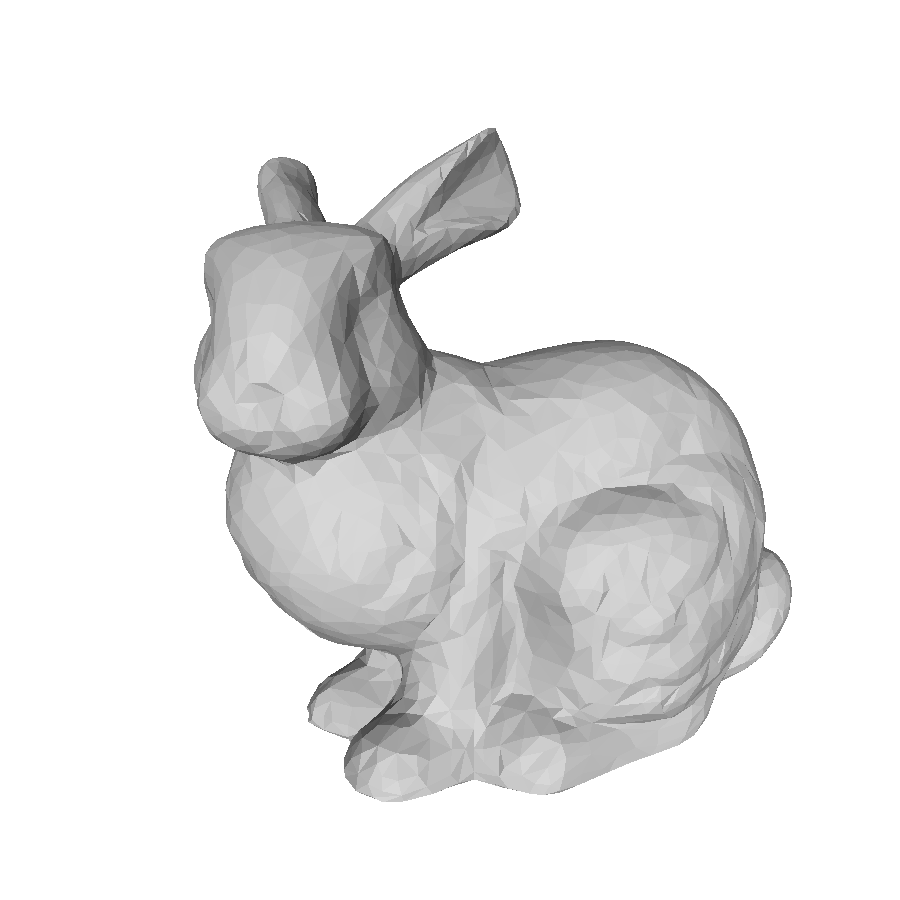
\includegraphics[width=0.66\textwidth, frame]{images/bunny_mesh.png}
	\caption{Mesh des Stanford Bunny \cite{stanfordbunny}}
	\label{fig:bunny_mesh}
\end{figure}

Vertices, Edges und Faces können in verschiedenen Repräsentationen gespeichert werden.
Diese haben unterschiedliche Eigenschaften und Vor- und Nachteile, die im folgenden genauer beleuchtet werden.
Zum besseren Verständnis wird das in \autoref{fig:triangles-example} dargestellte Polygonnetz jeweils in den unterschiedlichen Strukturen codiert.

\begin{figure}[ht]
\centering
\begin{tikzpicture}[scale=3]
\coordinate[label=-135:$v_1$] (v_1) at (0,0);
\coordinate[label=-45:$v_2$] (v_2) at (1,0);
\coordinate[label=135:$v_3$] (v_3) at (0,1);
\coordinate[label=45:$v_4$] (v_4) at (1,1);
\coordinate[label=$F_1$] (F_1) at (0.3,0.2);
\coordinate[label=$F_2$] (F_2) at (0.75,0.66);
\draw (v_1) to node[below]{$e_1$} (v_2);
\draw (v_2) to node[right]{$e_2$} (v_3);
\draw (v_3) to node[left]{$e_3$} (v_1);
\draw (v_2) to node[right]{$e_4$} (v_4);
\draw (v_4) to node[above]{$e_5$} (v_3);
\fill (v_1) circle (1pt);
\fill (v_2) circle (1pt);
\fill (v_3) circle (1pt);
\fill (v_4) circle (1pt);
\end{tikzpicture}
\caption{Beispielhaftes Polygonnetz, bestehend aus Knoten, Kanten und Facetten}
\label{fig:triangles-example}
\end{figure}

\subsection{\acl{VVM}}
\label{subsec:v-v-mesh}

Beim \ac{VVM} werden nur Vertices gespeichert, Kanten und Flächen ergeben sich implizit.
Zu den in \autoref{fig:triangles-example} dargestellten Dreiecken wird also die Liste in \autoref{tab:vvm-table} gespeichert.

\begin{table}[ht]
\centering
\begin{tabular}{| l | l |}
	\hline
	Vertex & verbundene Vertices\\
	\hline
	$v_1$ & $v_2, v_3$\\
	$v_2$ & $v_1, v_3, v_4$\\
	$v_3$ & $v_1, v_2, v_4$\\
	$v_4$ & $v_2, v_3$\\
	\hline
\end{tabular}
\caption{Vertextabelle beim \ac{VVM}}
\label{tab:vvm-table}
\end{table}

Der Speicherbedarf dieser simplen Darstellung ist sehr gering.
Die Einträge in der Tabelle können als Indizes der Vertexliste gespeichert werden.
Weiterhin sind Vertex-basierte Operationen sehr schnell.
Zum Hinzufügen eines Knotens muss beispielsweise nur ein neuer Eintrag in der Liste angelegt werden, sowie der neue Knoten zu den verbundenen Vertices hinzugefügt werden.

Um jedoch Informationen zu bestimmten Kanten oder Flächen zu bekommen, muss über die gesamte Liste iteriert werden.
Dies ist sehr langsam und schränkt den praktischen Nutzen von \acp{VVM} stark ein.

Ein Vergleich und eine Abwägung der Vor- und Nachteile mit anderen Datenstrukturen findet sich in \cite[Kap. 11]{smith2006vertex}.
Neben dem \ac{VVM} kann man in beliebigen Kombinationen auch Listen für Kanten oder Faces hinzufügen.
Dies erhöht zwar den Speicherbedarf und die Komplexität der Datenstruktur, bestimmte Zugriffe werden dadurch jedoch stark beschleunigt.


\subsection{Winged Edge}
\label{subsec:winged-edge}

In der Winged-Edge-Datenstruktur \cite{baumgart1975polyhedron} werden sowohl Vertices als auch Edges und Faces explizit abgespeichert.
Diese Repräsentation ermöglicht es, die Geometrie des Meshes im Vergleich zu anderen Strukturen leichter zu verändern.
Der Nachteil ist jedoch, dass der Speicheraufwand sehr hoch und die Datenstruktur im Vergleich zu den anderen Darstellungen sehr komplex ist.

\begin{figure}[ht]
\centering
\begin{tikzpicture}[scale=2]
\coordinate[label=45:$v_1$] (v_1) at (1,1);
\coordinate[label=135:$v_2$] (v_2) at (2,1);
\coordinate[label=-135:$v_3$] (v_3) at (0.5,2);
\coordinate[label=135:$v_4$] (v_4) at (0.5,0);
\coordinate[label=-45:$v_5$] (v_5) at (2.5,2);
\coordinate[label=45:$v_6$] (v_6) at (2.5,0);
\coordinate[label=$F_1$] (F_1) at (1.5,0.2);
\coordinate[label=$F_2$] (F_2) at (1.5,1.5);
\draw (v_1) to node[below]{$e$} (v_2);
\draw (v_1) to node[above right]{$\leftarrow\circlearrowleft$} (v_3);
\draw (v_1) to node[below right]{$\leftarrow\circlearrowright$} (v_4);
\draw (v_2) to node[above left]{$\rightarrow\circlearrowleft$} (v_5);
\draw (v_2) to node[below left]{$\rightarrow\circlearrowright$} (v_6);
\draw[dashed] (v_1) to (0,1.5);
\draw[dashed] (v_1) to (0,0.5);
\draw[dashed] (v_2) to (3,1.5);
\draw[dashed] (v_2) to (3,0.5);
\fill (v_1) circle (1pt);
\fill (v_2) circle (1pt);
\fill (v_3) circle (1pt);
\fill (v_4) circle (1pt);
\fill (v_5) circle (1pt);
\fill (v_6) circle (1pt);
\end{tikzpicture}
\caption{Vor- und Nachfolgerkanten der Winged-Edge-Datenstruktur (nach \cite[S.591]{baumgart1975polyhedron})}
\label{fig:winged-edge-edges}
\end{figure}

Bei der Winged-Edge-Darstellung werden in der Kantentabelle jeweils die vorhergehenden und nachfolgenden Kanten im und gegen den Uhrzeigersinn gespeichert.
Dies ermöglicht die schnelle Bestimmung von angrenzenden Kanten, Vertices oder Faces, bedeutet aber gleichzeitig auch viel Verwaltungsaufwand der Indizes.
In \autoref{fig:winged-edge-edges} findet sich eine Übersicht über die entsprechenden Kanten.

Die Winged-Edge-Datenstruktur zum Beispiel in \autoref{fig:triangles-example} ist in \autoref{tab:winged-edge-table} zu sehen.


\begin{table}[ht]
\centering
% Edges
\begin{tabular}{| l | l | l | l | l | l | l |}
\hline
\multicolumn{7}{| c |}{\textbf{Edges}}\\
\hline\hline
Edge & Vertices & Faces & $\leftarrow \circlearrowleft$ & $\leftarrow \circlearrowright$ & $\rightarrow \circlearrowleft$ & $\rightarrow \circlearrowright$\\
\hline
$e_1$ & $v_1, v_2$ & $F_1$ & $e_3$ & $e_3$ & $e_2$ & $e_4$\\
$e_2$ & $v_2, v_3$ & $F_1, F_2$ & $e_1$ & $e_4$ & $e_3$ & $e_5$\\
$e_3$ & $v_3, v_1$ & $F_1$ & $e_2$ & $e_5$ & $e_1$ & $e_1$\\
$e_4$ & $v_2, v_4$ & $F_2$ & $e_2$ & $e_1$ & $e_5$ & $e_5$\\
$e_5$ & $v_4, v_3$ & $F_2$ & $e_4$ & $e_4$ & $e_2$ & $e_3$\\
\hline
\multicolumn{7}{}{}\\
\cline{1-2}\cline{6-7}
\multicolumn{2}{| c |}{\textbf{Vertices}} & \multicolumn{3}{}{} & \multicolumn{2}{| c |}{\textbf{Faces}}\\
\cline{1-2}\cline{6-7}\noalign{\vskip\doublerulesep\vskip-\arrayrulewidth}\cline{1-2}\cline{6-7}
Vertex & Edges & \multicolumn{3}{c|}{} & Face & Edges\\\cline{1-2}\cline{6-7}
$v_1$ & $e_1, e_3$ & \multicolumn{3}{c|}{} & $F_1$ & $e_1, e_2, e_3$\\
$v_2$ & $e_1, e_2, e_4$ & \multicolumn{3}{c|}{} & $F_2$ & $e_4, e_5, e_2$\\\cline{6-7}
$v_3$ & $e_2, e_3, e_5$ & \multicolumn{5}{}{}\\
$v_4$ & $e_4, e_5$ & \multicolumn{5}{}{}\\\cline{1-2}
\end{tabular}
\caption{Vertex-, Edge- und Face-Tabellen bei der Winged-Edge-Darstellung}
\label{tab:winged-edge-table}
\end{table}


%TODO Half-edge
\subsection{Half Edge}
\label{subsec:half-edge}

Im Gegensatz zu bisherigen Modellen ist die Idee bei der Half-Edge-Datenstruktur, die Edges in jeweils zwei Halbkanten aufzuteilen.
Eine Halbkante hat somit einen Vor- und Nachfolger, sowie einen gegenüberliegenden Nachbarn.

Der Vorteil dieser Art der Speicherung ist, dass sowohl Kantenvorgänger und -nachfolger schnell bestimmt werden können, aber insbesondere auch aneinander angrenzende Faces. Das Hinzufügen, Entfernen oder Ändern von Daten ist jedoch leichter als bei der Winged-Edge-Darstellung, da nicht zu jeder Kante 4 Nachbarkanten und alle Faces gespeichert werden müssen.

\begin{table}[ht]
\centering
\begin{tabular}{| c | c | c | c | c |}
\hline
\multicolumn{5}{| c |}{\textbf{Edges}}\\
\hline
\hline
Edge & $\leftarrow$ Edge & $\rightarrow$ Edge & Origin & Face\\
\hline
$e_{1a}$ & $e_{3a}$ & $e_{2a}$ & $v_1$ & $F_1$\\
$e_{1b}$ & $e_{4b}$ & $e_{3b}$ & $v_2$ &     -\\
$e_{2a}$ & $e_{1a}$ & $e_{3a}$ & $v_2$ & $F_1$\\
$e_{2b}$ & $e_{5a}$ & $e_{4a}$ & $v_3$ & $F_2$\\
$e_{3a}$ & $e_{2a}$ & $e_{1a}$ & $v_3$ & $F_1$\\
$e_{3b}$ & $e_{1b}$ & $e_{5b}$ & $v_1$ &     -\\
$e_{4a}$ & $e_{2b}$ & $e_{5a}$ & $v_2$ & $F_2$\\
$e_{4b}$ & $e_{5b}$ & $e_{1b}$ & $v_4$ &     -\\
$e_{5a}$ & $e_{4a}$ & $e_{2b}$ & $v_4$ & $F_2$\\
$e_{5b}$ & $e_{3b}$ & $e_{4b}$ & $v_3$ &     -\\
\hline
\multicolumn{5}{}{}\\
\hline
\multicolumn{2}{| c |}{\textbf{Vertices}} & \multicolumn{3}{| c |}{\textbf{Faces}}\\
\hline\hline
Vertex & ausgehend & Face & Außenzyklus & Innenzyklus\\
\hline
$v_1$ & $e_{1a}, e_{3b}$ & $F_1$ & $e_{1b}, e_{3b}, e_{2b}$ & $e_{1a}, e_{2a}, e_{3a}$\\
$v_2$ & $e_{1b}, e_{2a}, e_{4a}$ & $F_2$ & $e_{4b}, e_{2a}, e_{5b}$ & $e_{2b}, e_{4a}, e_{5a}$\\
\cline{3-5}
$v_3$ & $e_{2b}, e_{3a}, e_{5b}$ & \multicolumn{3}{}{}\\
$v_4$ & $e_{4b}, e_{5a}$ & \multicolumn{3}{}{}\\
\cline{1-2}
\end{tabular}
\caption{Vertex-, Edge- und Face-Tabellen bei der Half-Edge-Darstellung}
\label{tab:half-edge-table}
\end{table}



\section{Point Cloud Library}
\label{sec:pcl}

Bei der \ac{PCL} \cite{rusu2011pcl} handelt es sich um eine Bibliothek, welche die Arbeit mit 3D-Punktwolken immens vereinfacht.
Sie bietet Möglichkeiten zur Filterung, Segmentierung, Oberflächenrekonstruktion und Visualisierung von Punktwolken, sowie weitere Module.

Neben den zahlreichen unterstützten Anwendungsgebieten und implementierten Algorithmen bietet die \ac{PCL} den weiteren entscheidenden Vorteil, dass sie direkt zu \ac{ROS} kompatibel ist.
Die Kompatibilität wird durch ROS-Nodelets im Paket \texttt{perception\_pcl} hergestellt, sodass Punktwolken, Meshes oder andere Datenstrukturen direkt per Message versendet werden können.
%TODO Relevanz?

% !TEX root = ../thesis.tex

\chapter{Vorhandene Arbeit}
\label{ch:vorhandene-arbeit}

In diesem Kapitel wird der aktuelle Stand der Forschung genannt sowie bereits existierende Lösungsansätze erklärt.


\section{Registrierung von Punktwolken}
\label{sec:registration}

\subsection{Lokale Registrierung}
\label{subsec:local-registration}

Bei der lokalen Registrierung von zwei Punktwolken müssen diese bereits grob aneinander ausgerichtet sein.
Der Registrierungsalgorithmus verfeinert diese Ausrichtung dann weiter.
Einer der bekanntesten Algorithmen zur lokalen Registrierung ist \ac{ICP} und seine vielen verschiedenen Varianten.


\subsubsection{\acl{ICP}}
\label{subsubsec:icp}

\ac{ICP} \cite{besl1992method} ist der wohl bekannteste Algorithmus zur lokalen Registrierung von Punktwolken.
Im Laufe der Zeit wurden zahlreiche Varianten und Optimierungen dafür entwickelt \cite{rusinkiewicz2001efficient, bouaziz2013sparse}.

Der Ansatz zur Registrierung der Punktwolke $A$ an der Punktwolke $B$ ist dabei der Folgende:
\begin{enumerate}
\item $A$ wird iterativ durch Anwendung von Translationen und Rotationen in eine neue Position gebracht, zum Beispiel mithilfe von Quaternionen \cite{horn1987closed}.
\item Zu jedem Punkt $p \in A$ wird der Punkt $q \in B$ gesucht, der den geringsten Abstand $\varepsilon$ von $p$ hat: $\varepsilon = \sqrt{(p_x - q_x)^2 + (p_y - q_y)^2 + (p_z - q_z)^2}$.
\item Standardmäßig wird nun als Fehler $e$ die Summe der Residuenquadrate verwendet: $e = \sum \varepsilon^2$
\item Wiederholung, bis eine der Abbruchbedingungen eintritt.
\end{enumerate}

Der Algorithmus terminiert, wenn:
\begin{itemize}
\item der Fehler $e$ unter einen Grenzwert fällt
\item $e$ bei erneuter Wiederholung nicht um einen bestimmten Wert sinkt
\item eine festgelegte Zahl von Iterationen abgelaufen ist.
\end{itemize}

Selbstverständlich lassen sich beliebig viele zusätzliche Abbruchbedingungen manuell definieren, beispielsweise eine festgelegte maximale Laufzeit.

\subsubsection{Kinect Fusion}
\label{subsubsec:kinfu}

Durch die Veröffentlichung der Microsoft Kinect im Jahr 2010 wurde aufgrund ihres niedrigen Preises erstmals der breiten Masse der Zugang zu Tiefenkameras ermöglicht \cite[1:55]{kinfuTalkYoutube}.
Die Kinect ist eine 3D-Kamera, welche ursprünglich für die Nutzung im Entertainment- und Gamingbereich entwickelt worden ist.
Bestehend aus einem Lichtemitter, Infrarotsensor, einer 2D-RGB-Kamera und weiteren Sensoren, liefert sie 3D-Daten bei einer Bildwiederholfrequenz von 30 Hz.
Neben dem ursprünglichen Anwendungsgebiet findet sie heute auch in vielen anderen, auch wissenschaftlichen Bereichen Anwendung, beispielsweise bei der Aufzeichnung geomorphologischer Daten \cite{mankoff2013kinect}.

\ac{KinFu} ist das Ergebnis einer Forschungsarbeit von Microsoft Research \cite{izadi2011kinectfusion} und bietet eine Möglichkeit, mithilfe der Kinect 3D-Rekonstruktionen in Echtzeit durchzuführen.
\ac{KinFu} kombiniert dabei die lokale Registrierung durch den \ac{ICP}-Algorithmus mit einem \ac{TSDF}.
Ein \ac{TSDF} ist im Grunde genommen nichts anderes als ein Voxel Grid.
Während  ein Voxel im ursprünglichen Voxel Grid entweder gefüllt ist oder nicht, wird hier die Entfernung zur nächsten Oberfläche gespeichert \cite{curless1996volumetric}.
Dies ermöglicht bei einer relativ geringen Voxelauflösung dennoch eine recht genaue Rekonstruktion der vorhandenen Oberflächen.
Um dies zu erreichen, werden die eingetragenen Werte interpoliert, und Fehler durch die geringe Auflösung so minimiert.

\begin{figure}[ht]
	\centering
	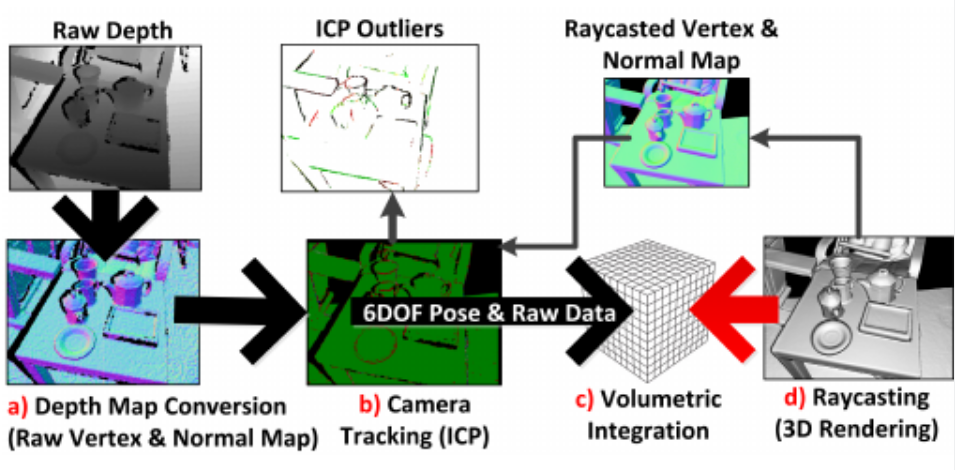
\includegraphics[width=0.66\textwidth, frame]{images/kinfu-integration.png}
	\caption{Integration eines Tiefenbilds in \ac{KinFu}. Entnommen aus \cite{izadi2011kinectfusion}}
	\label{fig:kinfu-integration}
\end{figure}

Durch eine schnelle GPU-Implementierung auf Basis von CUDA erreicht \ac{KinFu} dabei eine Integration neuer Tiefenbilder bei 30 Hz, der Bildwiederholfrequenz der Kinect.
Somit ist die zeitliche Differenz zwischen zwei Aufnahmen sehr niedrig.
Es wird davon ausgegangen, dass die Kamera handgeführt (bzw. mit geringer Geschwindigkeit bewegt) wird, daher hält sich auch die räumliche Distanz zwischen einzelnen Frames in Grenzen.
Aufgrund dieser Gegebenheiten reicht bei \ac{KinFu} eine lokale Registrierung aus, es kann also direkt \ac{ICP} verwendet werden.

In \autoref{fig:kinfu-integration} ist der Ablauf der Integration eines neuen Tiefenbilds ins \ac{TSDF} bei \ac{KinFu} dargestellt.
Das Tiefenbild wird zunächst in eine Punktwolke konvertiert.
Diese wird anschließend durch \ac{ICP} registriert, um dann unter Bildung eines Mittelwerts in das \ac{TSDF} integriert zu werden.
Zur Darstellung der Szene wird dieses anschließend mithilfe eines Raycasters gerendert.


% Hier YAK erwähnen und erklären
% YAK evtl. in Implementierung
Es gibt zahlreiche Optimierungen und veränderte Versionen von \ac{KinFu}.
Unter anderem gibt es in der \ac{PCL} eine freie Implementierung \cite{pirovano2012kinfu}.
Eine optimierte Version ist beispielsweise Chisel \cite{klingensmith2015chisel}, wo eine effizientere Voxelstrategie verwendet wird.
Weiterhin ist Chisel eine reine CPU-Implementierung, was die Nutzung auf Mobilgeräten ohne Grafikkarte ermöglicht.

Die in dieser Arbeit verwendete Implementierung ist \ac{YAK}.
\ac{YAK} ist eine auf \ac{ROS} angepasste Version von \ac{KinFu}, um Trajectory Waypoints für die Robotersteuerung zu errechnen \cite{schornak2019yak}.
Die Verwendung von \ac{KinFu} in industriellen Robotikanlagen ist in vielerlei Hinsicht sinnvoll:
\begin{itemize}
\item Objekte können aus mehreren Perspektiven gescannt werden, was eine bessere Darstellung der Szene liefert.
\item Rauschen durch den Bildsensor wird aufgrund der Mittelwertbildung minimiert.
Das Ergebnis ist ein glatteres und realistischeres Modell.
\item Durch die GPU-Implementierung können Tiefenbilder in Echtzeit integriert werden, was insbesondere bei Robotikanwendungen ein großer Vorteil ist.
\item Ein häufig in der Bildverarbeitung auftretendes Problem sind reflektierende bzw. spiegelnde Oberflächen.
Die betroffenen Regionen können oft nur falsch, verzerrt oder gar nicht modelliert werden.
Da hier eine Aufnahme aus mehreren Perspektiven möglich ist, können derartige Fehler weitestgehend vermieden werden. In \autoref{fig:yak-reflecting-model} ist dies an einem Beispiel besonders gut sichtbar.
\end{itemize}

\begin{figure}[ht]
	\centering
	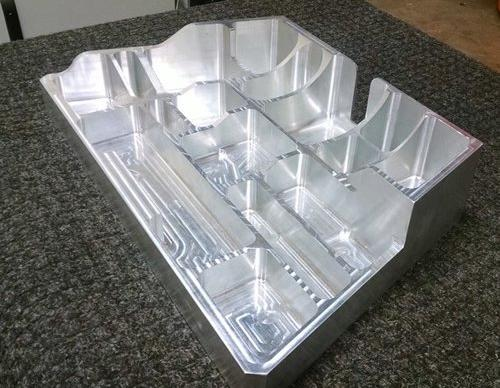
\includegraphics[width=0.4\textwidth]{images/yak-reflecting-scene.jpg}
	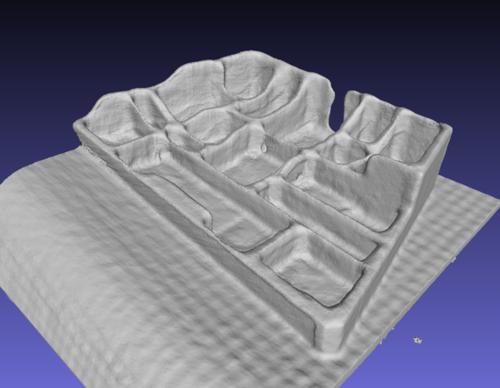
\includegraphics[width=0.4\textwidth]{images/yak-reflecting-reconstruction.png}
	\caption{Szene und Rekonstruktion eines reflektierenden Objekts durch \ac{YAK}. Entnommen aus \cite{schornak2019yak}}
	\label{fig:yak-reflecting-model}
\end{figure}


\subsection{Globale Registrierung}
\label{subsec:global-registration}

Bei der globalen Registrierung müssen sich die beiden Punktwolken nicht nahe der endgültigen Ausrichtung befinden - Translation und Rotation können beliebig sein.
Ein Nachteil ist jedoch, dass die globale Registrierung oft nur eine Grobregistrierung bietet, also keine optimalen Ergebnisse liefert.
Aus diesem Grund bietet es sich meist an, anschließend noch eine lokale Registrierung zur Verbesserung der Ergebnisse durchzuführen.

Zur globalen Registrierung von Punktwolken existieren verschiedene Ansätze \cite{chaudhury2015global, zhou2016fast, rusu2009fast}.
Die in dieser Arbeit verwendete Methode ist Super4PCS \cite{mellado2014super4pcs}, eine optimierte Version von \ac{4PCS} \cite{aiger2008fpcs}.
Dieser Ansatz wird verwendet, da die vorhandene Implementierung \ac{OpenGR} \cite{mellado2018opengr} über einen Wrapper bereits zur \ac{PCL} kompatibel ist.

%TODO 4PCS Funktionsweise erklären


\section{Segmentierung}
\label{sec:segmentation}

Ziel der Segmentierung ist es, zusammengehörende Bildregionen zu identifizieren und durch Zuweisung verschiedener Klassen voneinander zu trennen.
Dies ist, insbesondere in der 2D-Bildverarbeitung, ein altes Problem, für das es viele verschiedene Lösungsansätze gibt.
Auch im dreidimensionalen Raum ist eine Segmentierung häufig notwendig.
Häufig gibt es dabei nicht eine beste Methode - die Objektart, -größe, -form und viele weitere Faktoren beeinflussen die Wahl eines geeigneten Ansatzes.

Die Forschung ist in diesem Bereich weiterhin sehr aktuell:
Beispielsweise zeigen \citeauthor{uckermann2012real} einen Versuch, in Echtzeit und ohne vorher bekannte Objekte zu segmentieren \cite{uckermann2012real}.
Eine Übersicht bieten \citeauthor{nguyen20133d}, die verschiedene Varianten vergleichen und die Vor- und Nachteile diskutieren \cite{nguyen20133d}.
In den letzten Jahren findet auch verstärkt Forschung zur Segmentierung mithilfe von Neuronalen Netzen statt \cite{te2018rgcnn}.

% Segmentierung auf Meshes
Survey \cite{shamir2008survey}, SDF \cite{shapira2008consistent}


\section{Triangulierung}
\label{sec:triangulation}


\subsection{Marching Cubes}
\label{subsec:marching-cubes}
%TODO
Marching Cubes \cite{lorensen1987marching} \autoref{alg:marching-cubes}

\begin{algorithm}[ht]
\caption{Marching Cubes}
\label{alg:marching-cubes}
\begin{algorithmic}
\Function{marchingCubes}{}
	\State $vertexList \gets \emptyset$
	\Comment{The list of output triangles}
	\State $V \gets Voxels$
	\ForAll{$v \in V$}
		\State $index \gets$ \Call{calculateIndex}{v}
		\State $edgeList \gets edgeTable[index]$
		\ForAll{$edge \in edgeList$}
			\State $vertex \gets$ \Call{interpolate}{$edge[0], edge[1]$}
			\Comment{interpolate corners}
			\State \Call{$vertexList$.add}{$vertex$}
		\EndFor
	\EndFor
\EndFunction
\Function{calculateIndex}{$voxel$}
	\State $voxelIndex \gets 0$
	\For{$cornerIndex \in [0..8]$}
		\If{$voxel[cornerIndex] < isolevel$}
		\Comment{corner inside isosurface}
			\State $voxelIndex\ |=\ 1 << cornerIndex$
			\Comment{Set the i-th bit of the index}
		\EndIf
	\EndFor
	\State \Return{$voxelIndex$}
\EndFunction
\end{algorithmic}
\end{algorithm}


\subsection{Poisson}
\label{subsec:poisson}

%TODO
Poisson \cite{kazhdan2006poisson}


\subsection{Weitere Ansätze}
\label{subsec:triangulation-others}
%TODO Ball Pivot, Greedy Triangulation, (Delaunay?)
Greedy Projection \cite{Marton09ICRA},
Ball Pivoting \cite{bernardini1999ball}

% !TEX root = ../thesis.tex

\chapter{Implementierung}
\label{ch:implementierung}

Nachdem nun die theoretischen Grundlagen gelegt sind, wird im Folgenden die Implementierung der Pipeline erklärt.
Zunächst wird in \ref{sec:aufbau} der Aufbau des Programms beschrieben.
Die Interaktion und Parametrisierung wird in \ref{sec:interaktion} erläutert.
In \ref{sec:pipeline} wird dann der gesamte Ablauf der Pipeline und das Zusammenspiel der verschiedenen Komponenten noch einmal zusammengefasst.



\section{Aufbau}
\label{sec:aufbau}

Die Pipeline ist in C++ auf Basis der \ac{PCL} \cite{rusu2011pcl} geschrieben.
Dabei handelt es sich um eine Open-Source-Bibliothek, welche die Arbeit mit 3D-Punktwolken immens vereinfacht.
Sie bietet Möglichkeiten zur Filterung, Segmentierung, Oberflächenrekonstruktion und Visualisierung von Punktwolken, sowie weitere Module.

Neben den zahlreichen unterstützten Anwendungsgebieten und implementierten Algorithmen bietet die \ac{PCL} den weiteren entscheidenden Vorteil, dass sie direkt zu \ac{ROS} \cite{quigley2009ros} kompatibel ist.
Die Kompatibilität wird durch ROS-Nodelets im Paket \texttt{perception\_pcl} hergestellt, sodass Punktwolken, Meshes oder andere Datenstrukturen direkt zwischen \ac{ROS}-basierten Komponenten versendet werden können.

Um eine modulare Verwendung des Tools zu gewährleisten wurde ein einzelnes \ac{ROS}-Paket erstellt.
Die 3D-Datenverarbeitung findet hauptsächlich auf Basis der \ac{PCL} statt, mit einer Grobregistrierung über \ac{OpenGR}.
Zur 2D-Segmentierung über den Watershed-Algorithmus wird OpenCV verwendet.

Weiterhin werden eine aktuelle Version des Ensenso SDKs und die \ac{ROS}-Serviceheader zu den von Mikado versendeten Nachrichten benötigt.
Mit ihrer Hilfe können die aktuellen 2D-Grauwertbilder ausgelesen und zur Segmentierung verwendet werden.



\section{Interaktion und Parametrisierung}
\label{sec:interaktion}

Die Interaktion zwischen Mikado und dem Rekonstruktionstool findet über \ac{ROS} statt.
Dabei handelt es sich um einen \texttt{ros::Subscriber} auf das von Mikado veröffentlichte Topic \texttt{/point\_cloud}.
Bei Aufnahme einer neuen Punktwolke wird somit das Durchlaufen der Pipeline automatisch angestoßen.

Weiterhin lassen sich über \texttt{rosparam set} und \texttt{rosparam get} Parameter setzen oder auslesen.
Diese werden dann im Programm geparst und - falls nicht vorhanden - durch Standardwerte ersetzt.
Dies bietet mehrere Vorteile gegenüber anderen Optionen:

\begin{itemize}
\item Parameter können optional über die Konsole, auf Programmebene oder auch gar nicht gesetzt werden.
\item Das Programm muss nicht für jede Konfiguration neu kompiliert werden und kann bei Laufzeit parametrisiert werden.
\item Die Interaktion mit anderen Programmen ist durch die Verwendung der \ac{ROS}-Schnittstelle erheblich vereinfacht.
\end{itemize}

Auch die Triangulation wird durch einen externen Trigger angestoßen.
Dieser wird als \texttt{rosservice} zur Verfügung gestellt, welcher mit dem Output-Dateipfad aufgerufen wird.
Auch hier ist durch die Verwendung der \ac{ROS}-basierten Schnittstelle eine hohe Flexibilität gegeben.



\section{Pipelineablauf}
\label{sec:pipeline}

Der Ablauf der Pipeline ist stark abhängig von der durch den Nutzer gewählten Konfiguration.
Diese kann jedoch auch nach Start des Programms noch geändert werden.
Ohne vorherige Wahl eines Modus werden weder Segmentierung noch Registrierung vorgenommen.

\begin{figure}[H]
    \centering
	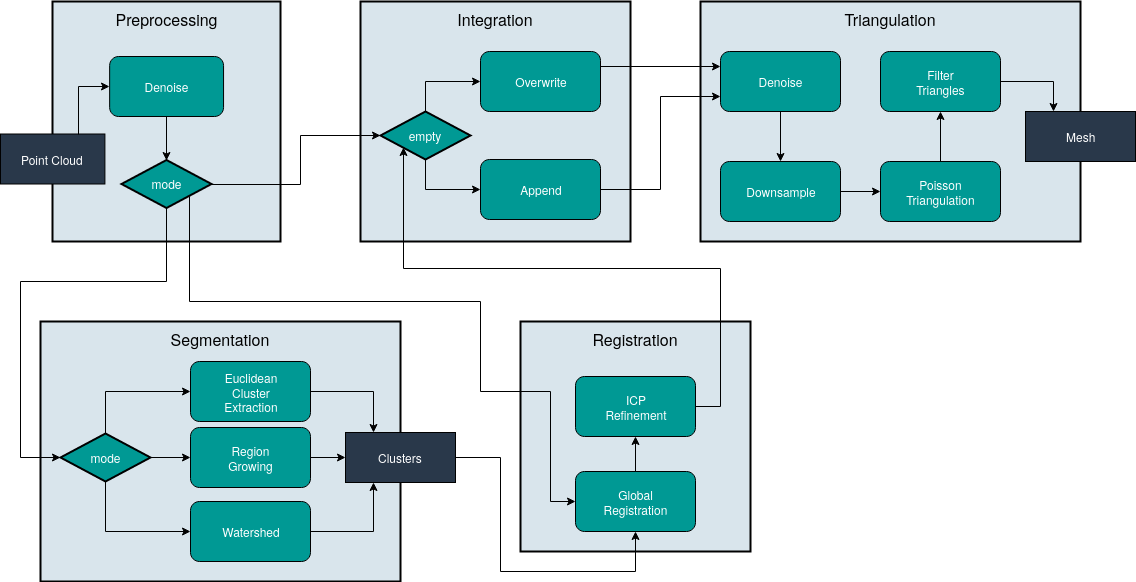
\includegraphics[width=\textwidth]{images/pipeline.png}
	\caption{Ablauf der Pipeline}
	\label{fig:pipeline}
\end{figure}

Der gesamte Ablauf des Prozesses vom Empfang einer Punktwolke bis zur Ausgabe des rekonstruierten Meshs ist in \autoref{fig:pipeline} sichtbar.
Der Programmablauf kann in mehrere verschiedene Blöcke unterteilt werden, welche im Folgenden erläutert werden.


\subsection{Preprocessing}
\label{subsec:pipeline-preprocessing}

Das Preprocessing findet unabhängig von der Wahl des Modus statt.
Nach Empfang einer Punktwolke wird diese zunächst durch ein \texttt{pcl::StatisticalOutlierRemoval} gefiltert.
Das Ziel ist die Eliminierung von unvermeidbarem Sensorrauschen.

In diesem Schritt könnten auch noch andere Preprocessingmethoden durchgeführt werden.
Dabei kann es sich sowohl um ein Downsampling zur Datenreduktion handeln als auch um Prozesse wie eine Normalenschätzung, falls diese nicht bereits vorher stattgefunden hat.


\subsection{Segmentierung}
\label{subsec:pipeline-segmentierung}

Dieser Block wird nur ausgeführt, wenn der entsprechende Modus gewählt ist.
In diesem Schritt findet die Segmentierung der Punktwolke statt.
Je nach gewählter Methode lässt sich dabei zwischen \ac{ECE}, Region Growing und Watershed-Segmentierung wählen.
Die Punktwolke wird dabei in einen Vektor gespalten, der die einzelnen Cluster beinhaltet.


\subsection{Registrierung}
\label{subsec:pipeline-registrierung}

Hier wird die Eingabepunktwolke an der bereits integrierten Punktwolke registriert.
Dabei wird zunächst eine globale Schätzung mithilfe von \ac{4PCS} durchgeführt.
Diese Registrierung wird anschließend durch \ac{ICP} verfeinert.

Der Registrierungsprozess wird abgebrochen, falls einer der beiden Registrierungen nicht konvergiert.
Weiterhin kann ein Grenzwert gewählt werden, unter dem der Score liegen muss.
Bei \ac{ICP} beschreibt dieser Score den \ac{MSE}.

Die Registrierung wird durch Parametrisierung aktiviert bzw. deaktiviert.
Hat zuvor eine Segmentierung stattgefunden, wird jeder Cluster seperat diesem Block zugeführt.


\subsection{Integration}
\label{subsec:pipeline-integration}

Dieser Schritt beschreibt das Zusammenführen der beiden Punktwolken.
Es wird vorausgesetzt, dass vorher bereits eine Registrierung stattgefunden hat.

In der Praxis ist dieser Block sehr einfach gehalten.
Liegt die Zahl der Punkte unter einem Grenzwert, werden diese überschrieben.
Ist dies nicht der Fall, müssen die beiden Vektoren konkateniert werden.


\subsection{Triangulierung}
\label{subsec:pipeline-triangulierung}

Entspricht die zusammengeführte Punktwolke den Erwartungen des Nutzers, kann dieser nun die Triangulierung anstoßen.
Dies bedeutet, dass dieser Block nicht automatisch ausgeführt wird.
Der Grund dafür ist, dass es sich um einen sehr zeit-, speicher- und rechenintensiven Vorgang handelt.

Zunächst findet eine weitere Filterung statt.
Dies ermöglicht selbst dann ein brauchbares Ergebnis, falls im Registrierungsschritt keine fehlerfreie Ausrichtung erreicht worden ist.
Im Optimalfall werden die fehlerhaften Daten aufgrund der hohen Punktdichte an der Oberfläche somit größtenteils entfernt.

Nach dem anschließenden Downsampling findet eine Poisson-Triangulierung statt.
Im letzten Schritt werden nun Dreiecke aus dem Polygonnetz entfernt, die über einer festgelegten Entfernung von der Punktwolke entfernt sind.
Da die Poisson-Triangulierung immer wasserdichte Polygone erzeugt, können auch inkorrekte Dreiecke generiert werden.
Diese werden hier entfernt.

% !TEX root = ../thesis.tex

\chapter{Auswertung}
\label{ch:auswertung}
% !TEX root = ../thesis.tex

\chapter{Fazit}
\label{ch:fazit}

%TODO

\cite{kazhdan2020poisson}
\nocite{*}

% ---------------------------------------------------------------------------
\newpage
\pagenumbering{Roman}
\setcounter{page}{\value{anhang}}
\printbibliography[heading=bibintoc]
% Include appendix and lists if needed
%% !TEX root = ../thesis.tex
\addcontentsline{toc}{chapter}{List of Figures}
\listoffigures
%% !TEX root = ../thesis.tex
\addcontentsline{toc}{chapter}{List of Tables}
\listoftables
%% !TEX root = ../thesis.tex
\addcontentsline{toc}{chapter}{List of Algorithms}
\listofalgorithms
%% !TEX root = ../thesis.tex
\begin{appendices}

\chapter{Proofs}


\chapter{Additional Figures}

\chapter{Additional Table}


\end{appendices}

\end{document}
